% ============================================================
% Question Bank: ch06-04 Constructing Triangles
% Topic Title: Constructing Triangles from Three Measurements
% CCSS: 7.G.A.2
% Questions: 27 (15 MC + 6 SA + 6 Graphical)
% ============================================================

% --- Multiple Choice Questions (15) ---

\begin{practiceQuestion}{6-4-q01}{mc}
\begin{questionText}
A triangle has sides $5$ cm, $7$ cm, and $11$ cm. How many triangles can be constructed with these exact measurements?
\end{questionText}
\choiceA{None}
\choiceB{Exactly one}
\choiceC{Exactly two}
\choiceD{Infinitely many}
\correctAnswer{B}
\explanation{Three given side lengths (SSS) that satisfy the triangle inequality produce exactly one unique triangle. Check: $5 + 7 = 12 > 11$, $5 + 11 = 16 > 7$, $7 + 11 = 18 > 5$. All conditions pass, so exactly one triangle exists.}
\end{practiceQuestion}

\begin{practiceQuestion}{6-4-q02}{mc}
\begin{questionText}
A triangle has angles $30°$, $70°$, and $80°$. How many triangles with different sizes can be drawn using these angle measures?
\end{questionText}
\choiceA{None}
\choiceB{Exactly one}
\choiceC{Exactly three}
\choiceD{Infinitely many}
\correctAnswer{D}
\explanation{Three angles (AAA) determine the shape of a triangle but not its size. Since no side length is fixed, infinitely many similar triangles of different sizes can be drawn with these angles.}
\end{practiceQuestion}

\begin{practiceQuestion}{6-4-q03}{mc}
\begin{questionText}
Can a triangle be formed with sides $3$ cm, $5$ cm, and $9$ cm?
\end{questionText}
\choiceA{Yes, because all side lengths are positive}
\choiceB{Yes, because it forms a scalene triangle}
\choiceC{No, because $3 + 5 = 8 < 9$}
\choiceD{No, because the sides are not equal}
\correctAnswer{C}
\explanation{By the triangle inequality theorem, the sum of any two sides must be greater than the third side. Here $3 + 5 = 8 < 9$, so the two shorter sides cannot reach across the longest side to form a triangle.}
\end{practiceQuestion}

\begin{practiceQuestion}{6-4-q04}{mc}
\begin{questionText}
Two sides of a triangle measure $10$ cm and $14$ cm with an included angle of $45°$. What triangle condition is this?
\end{questionText}
\choiceA{SSS}
\choiceB{SAS}
\choiceC{ASA}
\choiceD{AAA}
\correctAnswer{B}
\explanation{Two sides and the angle between them (the included angle) is the SAS (Side-Angle-Side) condition. SAS always determines a unique triangle.}
\end{practiceQuestion}

\begin{practiceQuestion}{6-4-q05}{mc}
\begin{questionText}
Which set of conditions does NOT always produce a unique triangle?
\end{questionText}
\choiceA{Three sides (SSS) satisfying the triangle inequality}
\choiceB{Two sides and the included angle (SAS)}
\choiceC{Two angles and the included side (ASA)}
\choiceD{Two sides and a non-included angle (SSA)}
\correctAnswer{D}
\explanation{SSA (two sides and a non-included angle) is the ambiguous case. It can produce zero, one, or two triangles depending on the measurements. SSS, SAS, and ASA each always produce exactly one unique triangle.}
\end{practiceQuestion}

\begin{practiceQuestion}{6-4-q06}{mc}
\begin{questionText}
Two angles of a triangle are $48°$ and $67°$. What is the measure of the third angle?
\end{questionText}
\choiceA{$55°$}
\choiceB{$65°$}
\choiceC{$75°$}
\choiceD{$115°$}
\correctAnswer{B}
\explanation{The sum of a triangle's interior angles is $180°$. The third angle is $180° - 48° - 67° = 65°$.}
\end{practiceQuestion}

\begin{practiceQuestion}{6-4-q07}{mc}
\begin{questionText}
Can a triangle have sides $7$, $7$, and $15$?
\end{questionText}
\choiceA{Yes, it is an isosceles triangle}
\choiceB{Yes, it is a right triangle}
\choiceC{No, the triangle inequality is violated}
\choiceD{No, two sides cannot be equal}
\correctAnswer{C}
\explanation{By the triangle inequality, $7 + 7 = 14 < 15$. The sum of the two shorter sides must exceed the longest side, so no triangle can be formed.}
\end{practiceQuestion}

\begin{practiceQuestion}{6-4-q08}{mc}
\begin{questionText}
You are given two angles ($65°$ and $45°$) and the side between them is $12$ cm. How many triangles can be constructed?
\end{questionText}
\choiceA{None}
\choiceB{Exactly one}
\choiceC{Exactly two}
\choiceD{Infinitely many}
\correctAnswer{B}
\explanation{This is the ASA (Angle-Side-Angle) condition. Two angles and the included side always determine exactly one unique triangle.}
\end{practiceQuestion}

\begin{practiceQuestion}{6-4-q09}{mc}
\begin{questionText}
A right triangle has legs $a$ and $b$. If one leg is $6$ cm and the hypotenuse is $10$ cm, what is the other leg?
\end{questionText}
\choiceA{$4$ cm}
\choiceB{$6$ cm}
\choiceC{$8$ cm}
\choiceD{$16$ cm}
\correctAnswer{C}
\explanation{By the Pythagorean theorem, $a^2 + b^2 = c^2$. So $6^2 + b^2 = 10^2$, which gives $36 + b^2 = 100$, so $b^2 = 64$ and $b = 8$ cm.}
\end{practiceQuestion}

\begin{practiceQuestion}{6-4-q10}{mc}
\begin{questionText}
Which set of three side lengths can form a triangle?
\end{questionText}
\choiceA{$1$, $2$, $4$}
\choiceB{$3$, $6$, $10$}
\choiceC{$5$, $5$, $10$}
\choiceD{$4$, $6$, $9$}
\correctAnswer{D}
\explanation{Apply the triangle inequality to each set. For $4$, $6$, $9$: $4 + 6 = 10 > 9$ \checkmark, $4 + 9 = 13 > 6$ \checkmark, $6 + 9 = 15 > 4$ \checkmark. The other sets fail: $1 + 2 = 3 < 4$; $3 + 6 = 9 < 10$; $5 + 5 = 10 \not> 10$.}
\end{practiceQuestion}

\begin{practiceQuestion}{6-4-q11}{mc}
\begin{questionText}
A triangle has angles $90°$, $45°$, and $45°$. What type of triangle is this?
\end{questionText}
\choiceA{Equilateral}
\choiceB{Right scalene}
\choiceC{Right isosceles}
\choiceD{Obtuse isosceles}
\correctAnswer{C}
\explanation{A $90°$-$45°$-$45°$ triangle has one right angle (making it a right triangle) and two equal angles of $45°$ (making it isosceles). So it is a right isosceles triangle.}
\end{practiceQuestion}

\begin{practiceQuestion}{6-4-q12}{mc}
\begin{questionText}
Marcus tries to construct a triangle with sides $8$ cm, $15$ cm, and $6$ cm. What will happen?
\end{questionText}
\choiceA{He will form exactly one triangle}
\choiceB{He will form exactly two triangles}
\choiceC{He cannot form a triangle}
\choiceD{He will form an equilateral triangle}
\correctAnswer{C}
\explanation{By the triangle inequality, the sum of the two shorter sides must exceed the longest side. Here $6 + 8 = 14 < 15$, so the inequality fails and no triangle can be formed.}
\end{practiceQuestion}

\begin{practiceQuestion}{6-4-q13}{mc}
\begin{questionText}
Priya constructs a triangle with two sides of $9$ cm each and an included angle of $60°$. What type of triangle does she get?
\end{questionText}
\choiceA{Scalene}
\choiceB{Isosceles (not equilateral)}
\choiceC{Equilateral}
\choiceD{Right}
\correctAnswer{C}
\explanation{With SAS where both sides are equal ($9$ cm) and the included angle is $60°$, the triangle must be equilateral. An isosceles triangle with a $60°$ angle between the equal sides has all three angles equal to $60°$ and all three sides equal to $9$ cm.}
\end{practiceQuestion}

\begin{practiceQuestion}{6-4-q14}{mc}
\begin{questionText}
How many different triangles can be formed with angle measures $60°$, $60°$, and $60°$?
\end{questionText}
\choiceA{None}
\choiceB{Exactly one}
\choiceC{Exactly three}
\choiceD{Infinitely many}
\correctAnswer{D}
\explanation{When only angle measures are known (AAA), the shape is fixed but the size is not. Equilateral triangles of any size have angles $60°$-$60°$-$60°$, so infinitely many are possible.}
\end{practiceQuestion}

\begin{practiceQuestion}{6-4-q15}{mc}
\begin{questionText}
Kayla has side lengths $7$ cm and $10$ cm. Which third side length would make it impossible to form a triangle?
\end{questionText}
\choiceA{$4$ cm}
\choiceB{$8$ cm}
\choiceC{$12$ cm}
\choiceD{$18$ cm}
\correctAnswer{D}
\explanation{By the triangle inequality, the third side must be less than $7 + 10 = 17$ and greater than $10 - 7 = 3$. A side of $18$ cm is greater than $17$, so no triangle can be formed.}
\end{practiceQuestion}

% --- Short Answer Questions (6) ---

\begin{practiceQuestion}{6-4-q16}{sa}
\begin{questionText}
A triangle has angles $52°$ and $73°$. What is the measure of the third angle?
\end{questionText}
\correctAnswer{$55°$}
\explanation{The angle sum property states that interior angles of a triangle sum to $180°$. The third angle is $180° - 52° - 73° = 55°$.}
\end{practiceQuestion}

\begin{practiceQuestion}{6-4-q17}{sa}
\begin{questionText}
Two sides of a triangle are $11$ cm and $4$ cm. What is the range of possible lengths for the third side?
\end{questionText}
\correctAnswer{Greater than $7$ cm and less than $15$ cm}
\explanation{By the triangle inequality, the third side must be greater than $|11 - 4| = 7$ and less than $11 + 4 = 15$. So the third side must satisfy $7 < s < 15$.}
\end{practiceQuestion}

\begin{practiceQuestion}{6-4-q18}{sa}
\begin{questionText}
Leo is given sides $13$ cm, $5$ cm, and $7$ cm. Can he construct a triangle? Explain why or why not.
\end{questionText}
\correctAnswer{No}
\explanation{By the triangle inequality, the sum of any two sides must exceed the third. Check: $5 + 7 = 12 < 13$. Since $12$ is less than $13$, the two shorter sides are too short to form a triangle.}
\end{practiceQuestion}

\begin{practiceQuestion}{6-4-q19}{sa}
\begin{questionText}
A triangle has two angles that each measure $55°$. Is this triangle isosceles, equilateral, or scalene?
\end{questionText}
\correctAnswer{Isosceles}
\explanation{The third angle is $180° - 55° - 55° = 70°$. Since two angles are equal ($55°$ each), the sides opposite those angles are also equal, making the triangle isosceles.}
\end{practiceQuestion}

\begin{practiceQuestion}{6-4-q20}{sa}
\begin{questionText}
Dana is given sides $8$ cm, $8$ cm and an included angle of $90°$. How many unique triangles can she construct?
\end{questionText}
\correctAnswer{$1$}
\explanation{The SAS condition (two sides and the included angle) always determines exactly one unique triangle. With sides $8$, $8$ and an included angle of $90°$, she constructs one right isosceles triangle.}
\end{practiceQuestion}

\begin{practiceQuestion}{6-4-q21}{sa}
\begin{questionText}
In a triangle, one angle measures $120°$ and a second angle measures $35°$. What is the third angle, and classify the triangle as acute, right, or obtuse.
\end{questionText}
\correctAnswer{$25°$; obtuse}
\explanation{The third angle is $180° - 120° - 35° = 25°$. Because one angle ($120°$) is greater than $90°$, the triangle is classified as obtuse.}
\end{practiceQuestion}

% --- Graphical MC Questions (3) ---

\begin{practiceQuestion}{6-4-q22}{gmc}
\begin{questionText}
Examine the triangle below. Which condition describes the information shown?

\begin{center}
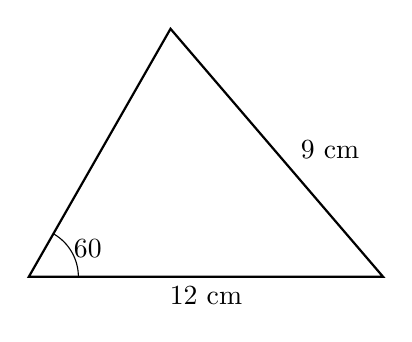
\begin{tikzpicture}[scale=0.9]
  \coordinate (A) at (0,0);
  \coordinate (B) at (5,0);
  \coordinate (C) at (2,3.5);
  \draw[thick] (A) -- (B) -- (C) -- cycle;
  % side labels
  \node[below] at (2.5,0) {$12$ cm};
  \node[right] at (3.7,1.8) {$9$ cm};
  % angle at A
  \draw (0.7,0) arc[start angle=0,end angle=60,radius=0.7];
  \node[right] at (0.5,0.4) {$60°$};
\end{tikzpicture}
\end{center}
\end{questionText}
\choiceA{SSS}
\choiceB{SAS}
\choiceC{ASA}
\choiceD{AAA}
\correctAnswer{B}
\explanation{The diagram shows two side lengths ($12$ cm and $9$ cm) and the angle between them ($60°$). This is the SAS (Side-Angle-Side) condition, which always produces a unique triangle.}
\end{practiceQuestion}

\begin{practiceQuestion}{6-4-q23}{gmc}
\begin{questionText}
Look at the three segments below. Can they form a triangle?

\begin{center}
\begin{tikzpicture}[scale=0.8]
  \draw[thick,funBlue] (0,0) -- (2,0);
  \node[below] at (1,0) {$2$ cm};
  \draw[thick,funRed] (0,-1) -- (3,-1);
  \node[below] at (1.5,-1) {$3$ cm};
  \draw[thick,funGreen] (0,-2) -- (6,-2);
  \node[below] at (3,-2) {$6$ cm};
\end{tikzpicture}
\end{center}
\end{questionText}
\choiceA{Yes, because all lengths are positive}
\choiceB{Yes, because there are exactly three segments}
\choiceC{No, because $2 + 3 = 5 < 6$}
\choiceD{No, because the segments are different colors}
\correctAnswer{C}
\explanation{By the triangle inequality theorem, the sum of any two sides must be greater than the third side. Here $2 + 3 = 5 < 6$, so the two shorter segments cannot meet to close the triangle.}
\end{practiceQuestion}

\begin{practiceQuestion}{6-4-q24}{gmc}
\begin{questionText}
The triangle below has the measurements shown. How many unique triangles can be constructed with this information?

\begin{center}
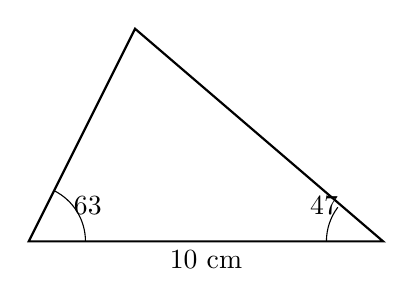
\begin{tikzpicture}[scale=0.9]
  \coordinate (A) at (0,0);
  \coordinate (B) at (5,0);
  \coordinate (C) at (1.5,3);
  \draw[thick] (A) -- (B) -- (C) -- cycle;
  % angle at A
  \draw (0.8,0) arc[start angle=0,end angle=63,radius=0.8];
  \node[right] at (0.5,0.5) {$63°$};
  % angle at B
  \draw (4.2,0) arc[start angle=180,end angle=143,radius=0.8];
  \node[left] at (4.5,0.5) {$47°$};
  % side AB
  \node[below] at (2.5,0) {$10$ cm};
\end{tikzpicture}
\end{center}
\end{questionText}
\choiceA{None}
\choiceB{Exactly one}
\choiceC{Exactly two}
\choiceD{Infinitely many}
\correctAnswer{B}
\explanation{The diagram shows two angles and the side between them (ASA condition): $63°$, $47°$, and the included side of $10$ cm. ASA always determines exactly one unique triangle.}
\end{practiceQuestion}

% --- Graphical SA Questions (3) ---

\begin{practiceQuestion}{6-4-q25}{gsa}
\begin{questionText}
Use the triangle below. Find the measure of the missing angle $x$.

\begin{center}
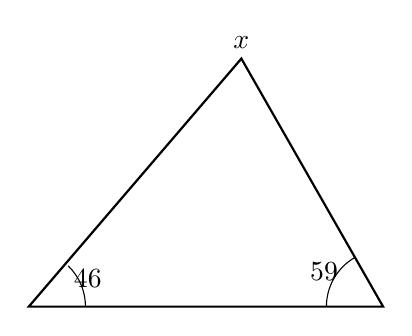
\begin{tikzpicture}[scale=0.9]
  \coordinate (A) at (0,0);
  \coordinate (B) at (5,0);
  \coordinate (C) at (3,3.5);
  \draw[thick] (A) -- (B) -- (C) -- cycle;
  % angle at A
  \draw (0.8,0) arc[start angle=0,end angle=46,radius=0.8];
  \node[right] at (0.5,0.4) {$46°$};
  % angle at B
  \draw (4.2,0) arc[start angle=180,end angle=120,radius=0.8];
  \node[left] at (4.5,0.5) {$59°$};
  % angle at C
  \node[above] at (3,3.5) {$x°$};
\end{tikzpicture}
\end{center}
\end{questionText}
\correctAnswer{$75°$}
\explanation{The sum of interior angles in a triangle is $180°$. So $x = 180° - 46° - 59° = 75°$.}
\end{practiceQuestion}

\begin{practiceQuestion}{6-4-q26}{gsa}
\begin{questionText}
Determine whether the three segments shown below can form a triangle. If yes, state what type (scalene, isosceles, or equilateral). If no, explain why.

\begin{center}
\begin{tikzpicture}[scale=0.7]
  \draw[thick,funBlue] (0,0) -- (4,0);
  \node[below] at (2,0) {$8$ cm};
  \draw[thick,funRed] (0,-1) -- (4,-1);
  \node[below] at (2,-1) {$8$ cm};
  \draw[thick,funGreen] (0,-2) -- (4,-2);
  \node[below] at (2,-2) {$8$ cm};
\end{tikzpicture}
\end{center}
\end{questionText}
\correctAnswer{Yes; equilateral}
\explanation{All three sides are $8$ cm. Check triangle inequality: $8 + 8 = 16 > 8$ \checkmark. Since all three sides are equal, the triangle is equilateral.}
\end{practiceQuestion}

\begin{practiceQuestion}{6-4-q27}{gsa}
\begin{questionText}
The diagram shows a triangle with two known angle measures and one unknown side. Find the missing angle and determine whether the given measurements produce a unique triangle.

\begin{center}
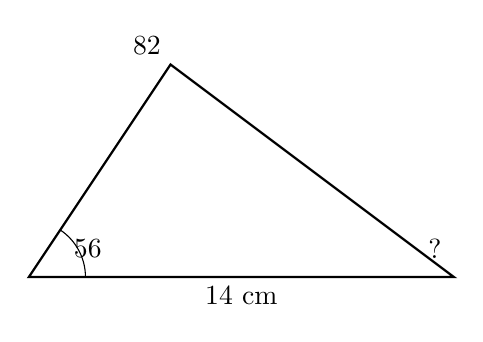
\begin{tikzpicture}[scale=0.9]
  \coordinate (A) at (0,0);
  \coordinate (B) at (6,0);
  \coordinate (C) at (2,3);
  \draw[thick] (A) -- (B) -- (C) -- cycle;
  % angle at A
  \draw (0.8,0) arc[start angle=0,end angle=56,radius=0.8];
  \node[right] at (0.5,0.4) {$56°$};
  % angle at C
  \node[above left] at (2,3) {$82°$};
  % side AB
  \node[below] at (3,0) {$14$ cm};
  % angle at B = ?
  \node[right] at (5.5,0.4) {$?$};
\end{tikzpicture}
\end{center}
\end{questionText}
\correctAnswer{$42°$; yes, unique triangle}
\explanation{The missing angle is $180° - 56° - 82° = 42°$. With two angles and the included side known (ASA), exactly one unique triangle can be constructed.}
\end{practiceQuestion}
